\documentclass[a4paper,11pt]{article}
\usepackage{a4wide}
\usepackage[ansinew]{inputenc}
\usepackage{graphicx}
\usepackage{bm}
\usepackage{natbib}
\usepackage{longtable}
\usepackage{rotating}
\usepackage{pdflscape}

%\usepackage{jurabib}
   %\jurabibsetup{  
     %authorformat=and  
    % commabeforerest,  
    % titleformat=colonsep,  
    % bibformat=tabular  
   %}  

\usepackage[bookmarks=true, bookmarksopen=true,
                bookmarksnumbered=true, colorlinks,citecolor = blue,
                filecolor=blue, linkcolor=blue, urlcolor=blue,
                plainpages=false,hyperindex=true]{hyperref}
\hypersetup{
        pdftitle={},
        pdfauthor={Anton Burger and Robert Ferstl},
        pdfsubject={},
        pdfkeywords={},
        pdfcreator={},
        pdfproducer={}
     }

%\usepackage{natbib}
%\usepackage{dingbat}
\usepackage{amssymb,amsmath,amstext}
%\usepackage{manfnt}

\setlength{\parindent}{0.0cm}                      % Absatzeinr�ckungen
\setlength{\parskip}{1.5ex plus 0.5ex minus 0.5ex} % Absatzabst�nde
%\renewcommand{\arraystretch}{1.5}                 % Zeilenabstand in Tabellen


\begin{document}
\title{Generation Capacity Investment in \\Electricity Markets under Uncertainty\thanks{available online at \href{http://www.ssrn.com}{http://www.ssrn.com}}}
\author{Anton Burger\thanks{\href{http://www.wu-wien.ac.at/regulierung}{Institute for Regulatory Economics, Vienna University of Economics and Business Administration,} \href{mailto:anton.burger@wu-wien.ac.at}{anton.burger@wu-wien.ac.at}}\hspace{1cm} Robert Ferstl\thanks{\href{http://www-finanzierung.uni-regensburg.de/}{Department of Finance, University of Regensburg,} \href{mailto:robert.ferstl@wiwi.uni-regensburg.de}{robert.ferstl@wiwi.uni-regensburg.de}}}
\maketitle

%\abstract{
The paper discusses a game theoretic model for generation capacity investment decisions in a deregulated electricity market. We use a node-based formulation of a multi-stage stochastic program. The uncertainty is modeled as stochastic demand function with a random intercept for different states of the market. We present a practical application of this $S$-adapted Cournot equilibrium, were we use data from the German electricity market.
\\
\\
\par
\textbf{Keywords:} electricity markets, stochastic oligopoly models, dynamic games
\\

\textbf{JEL Codes:} D43, L51
}


%%% Local Variables: 
%%% mode: plain-tex
%%% TeX-master: "gencapinvest"
%%% End: 

%\section{Introduction}

In this paper we will build a model for generation capacity investment under uncertainty. We consider a deregulated electricity market, where typically several large players act on market leading to an oligopoly situation. There is not much literature which directly deals with the question of  generation capacity investments. Recent works are \cite{Chuang2001}, \cite{Ventosa2002}, \cite{Chaton2003}, \cite{Hogendorn2003}, \cite{Pineau2003}, \cite{Ehrenmann2004}. \cite{Murphy2005}, \cite{Kiesling2007}, \cite{Pineau2007}.


Cournot is more flexible and better computational tractability.

\subsection{The Austrian electricity market}

approximately half page about Austrian electricity market: total consumption, major players, progress of deregulation, major generation technologies, competitive fringe, types of trades in the market


\subsection{Stochastic oligopoly models}

\textbf{References:} \cite{Salant1982, Wolf1997, Haurie2002, Pineau2003, Murto2004}\\


The $S$-adapted information structure was introduced by \cite{Haurie1990}.
$S$-adapted structure is similar to the open-loop case, except that the strategies of the players adapt to the sample path of the stochastic variable \citep[see][pg. 128]{Pineau2003}.

\cite{Haurie2002} developed an approximation method with variational inequalities for $S$-adapted oligopoly equilibria. It can be used with any discrete state process that can be represented as an event tree can be used as description of the random disturbances.

\cite{Murto2004} solves the game with feedback information structure.

\subsection{Short-term assumption for decision variables}

Cournot, Bertrand, SFE


In theory, the output of a competitive generation market is equal to the output of a regulated system with a central planner that minimizes investment plus operating costs to meet demand (Green, 2000), see \citep[see][pg. 111]{Rothwell2003}.

Papers with focus investment problem: \cite{Pineau2003}, \cite{Murphy2005}, \cite{Genc2007}, \cite{Kiesling2007}, \cite{Barmack2007}, \cite{Sauma2006}

Market simulation: \cite{Torre2003}, \cite{Valenzuela2007}, \cite{Hobbs2001},\cite{Otero-Novas2000}

General review paper: \cite{Neuhoff2005}, \cite{Ventosa2005}, \cite{Kahn1998}

%%% Local Variables: 
%%% mode: latex
%%% TeX-master: "../emarket_simulation"
%%% End: 

\section{Model}

\subsection{Overview}

In this section, we develop a stochastic dynamic equilibrium model for a deregulated electricity market. Our focus lies on studying the long-run economic effects of strategic investment decisions in different generation technologies. In each time step, the market-clearing conditions lead to the solution of a Nash-Cournot equilibrium between the oligopolistic market players. The uncertainty is modeled with a scenario tree for the stochastic inverse demand function with a random intercept. Further, we include probabilities for different market states. By deriving the Karush-Kuhn-Tucker (KKT) conditions for each subproblem, we can solve the model as mixed complementarity problem (MCP) and calibrate it to data from the German electricity market.


\subsection{Sample-path adapted open-loop}
\label{sec:sample-path-adapted}

\textbf{References}: \cite{Pineau2003}

Their solutions approach uses variational inequalities (VI). The model is similar to Games with Expected Scenarios (GES) in \cite{Genc2007}. The players assume that the future will evolve according to some expected values

\subsection{Notation}

\textbf{References:} \cite{Genc2007}, \cite{Genc2008}

\cite{Genc2007} concluded that the GPS formulation is the most appropriate one, and continue to use it in \cite{Genc2008}.
The players are aware of the uncertainty and account for it during the decision making process.

\cite{Genc2008} solve a stochastic programming model with six stages. They argue that more stages would have been appropriate, but the PATH solver was not able to handle more. They used hourly data for the demand and transformed it to daily values by simple averaging.

\begin{longtable}[l]{l l}
$i \in N$ & players, firms \\
$j \in M$ & technologies \\
$t \in T$ & time \\
$s \in S$ & scenarios \\
$p_s$ & probability of scenario $s$\\
$ q_{i,s}^{j,t}$ & production quantities \\
$I_{i,s}^{j,t}$ & investment quantities \\
$K_{i,s}^{j,t}$ & available capacity\\
$F^{j,t}$ & installment cost\\
$Q_s^t = \sum_{i\in N}\sum_{j\in M} q_{i,s}^{j,t}$ & market demand \\
$P_s^t$ & market equilibrium price \\
$\alpha_s^t$ & intercept of demand function \\
$\beta$ & slope of demand function \\
$c_j$ & variable costs \\
$\Pi_{i,s}^t$ & profit of player $i$ in scenario $s$ in time $t$\\
$\Pi_i^t = \sum_{s\in S}p_s\Pi_{i,s}^t$ & total profit of player $i$ in time $t$\\
$\delta_t$ & discount factor \\
$\nu$ & salvage value parameter\\
$r$ & depreciation rate\\
$\overline{P}_t$ & price cap\\ 

\end{longtable}

\begin{equation}
\Pi_{i,s}^t = \left(\alpha_s^t-\beta Q_s^t \right)\sum_{j\in M}q_{i,s}^{j,t}-\sum_{j\in M}c_jq_{i,s}^{j,t}
\end{equation}

Each player $i$ maximizes the discounted expected profit:

\begin{equation}
  \label{eq:objfct}
  \max_{q_{i,s}^{j,t}, I_{i,s}^{j,t}} \sum_{s\in S}p_s \sum_{t\in T}\delta_t \sum_{j\in J}\left[\Pi_{i,s}^t\left(q_{i,s}^{j,t}, I_{i,s}^{j,t}, K_{i,s}^{j,t}, Q_s^t\right) \right ]+ \sum_{s\in S}p_s\,\delta_T \sum_{j\in M}\left[K_{i,s}^{j,T}F^{j,T}\nu\right]
\end{equation}

subject to
  
\begin{eqnarray}  
q_{i,s}^{j,t} - K_{i,s}^{j,t} &\leq& 0 \quad \forall i,s,j,t \label{eq:prodconstr} \\
Q_s^t-\sum_{i\in N}\sum_{j\in M} q_{i,s}^{j,t} &=& 0 \quad \forall s,t \label{eq:marketclearing}\\
K_{i,s}^{j,t+1} - (1-r)K_{i,s}^{j,t}-I_{i,s}^{j,t} &=& 0 \quad \forall i,s,j,t \label{eq:state} \\
I_{i}^{j,t}-\sum_{s\in S}p_sI_{i,s}^{j,t} &=& 0 \quad \forall i,s,j,t \label{eq:nonant}\\
P_t^s - \overline{P}_t &\leq& 0 \quad \forall s,t \label{eq:pricecap}\\
-\sum_{s\in S}p_s \sum_{t\in T}\delta_t\left[\min\left(\overline{P}_t,P_t^s\right) -\sum_{j\in M}\left(c_jq_{i,s}^{j,t}\right)+\sum_{j\in M}\left(F^{j,t}I_{i,s}^{j,t}\right)\right]\\
  -\sum_{s\in S}p_s\,\delta_T \sum_{j\in M}\left[K_{i,s}^{j,T}F^{j,T}\nu\right] &\leq& 0 \quad \forall i\\
q_{i,s}^{j,t}, K_{i,s}^{j,t}, I_{i,s}^{j,t}  &\geq& 0 \quad \forall i,s,j,t\label{eq:nonneg}
\end{eqnarray}

\eqref{eq:prodconstr} is the production constraint, \eqref{eq:marketclearing} the market clearing condition, \eqref{eq:state} is the state equation, \eqref{eq:nonant} is the non-anticipativity constraint, \eqref{eq:pricecap} price cap, \eqref{eq:nonneg} are non-negativity constraints. The objective function \eqref{eq:objfct} consists of the expected discounted profits and the salvage values at the final stage of the planning horizon.

The cost functions are convex and twice-contiuous differentiable.

Market demand is characterized by the following price-quantity relationship:

\begin{equation}
  \label{eq:marketdemandpq}
  aP_t+bQ_t=D_t+\tilde{\gamma}_t, \quad \mbox{where}\, \tilde{\gamma}_t\sim\mathbb{N}(\mu,h)
\end{equation}

such that

\begin{eqnarray*}
  \label{eq:3}
  \tilde{\gamma}_0=0\qquad\mbox{for}\, t=0\\
   \tilde{\gamma}_t=\left\{\mp(2w-1)\gamma_t\right\}_{w=1}^{2^{t-1}}\\
   \gamma_t=\frac{h}{\sqrt{2^{1-t}\sum_{w=1}^{2^{t-1}}(2w-1)^2}}
\end{eqnarray*}

The demand is given by:

\begin{equation}
  \label{eq:demandgrowth}
  D_t = D(1+\rho_e)^t
\end{equation}

where $D>0$ and $\rho_e$ is the demand growth rate for the state $e$ ("high" growth, "low" growth, etc.). The demand follows a normal distribution in each time period. Therefore, \cite{Genc2008} assume that load is normally distributed with $\mathbb{N}(\mu, h^2)$.

Where $\mu=18,055$ MW and $p=48.2$. With a reduced-form electricity demand of

\begin{equation}
  \label{eq:5}
  Q_t(p) = \alpha_t-\beta p, 
\end{equation}

they calculate $\beta=75$ as follows:

\begin{eqnarray*}
  \frac{\partial Q_t(p)}{\partial p} &=& -\beta \\
  \frac{\partial Q_t(p)}{\partial p}\times\frac{Q}{p} &=& -\beta\times\frac{Q}{p} \\
  0.2 &=& -\beta\times\frac{18,055}{48.2}\\
\beta &=& 74.91701
\end{eqnarray*}


Let

\begin{equation*}
  \alpha_t=D(1+\rho_e)^t+\gamma_t,
\end{equation*}

with $\rho_e = \left\{0.006, 0.009, 0.013\right\}$ as yearly growth rates of demand for the future. For $\tilde{\gamma}_0=0$ we get

\begin{eqnarray*}
  18,055 &=& \alpha_0-75\times 48.2\\
  \alpha_0 &=&D=21,670.
\end{eqnarray*}

So, the demand curve in the initial node is $Q_o(p) = 21,670-75p$.

The intercept for 


\subsection{Solution}
\label{sec:solution}

% In general, the Karush-Kuhn-Tucker (KKT) conditions for mixed equality and inequality constraints are as follows:

% To maximize $f(\bm{x})$ with $\bm{x}=(x_1,\dots, x_n)$ subject to

% \begin{equation*}
%   g_1(\bm{x})\leq b_1, \quad\cdots\quad, g_k(\bm{x})\leq b_k,\qquad i=,1\dots, k
% \end{equation*}
% and

% \begin{equation*}
%   h_1(\bm{x})= c_1, \quad\cdots\quad, h_m(\bm{x})= c_m,\qquad j=,1\dots, m
% \end{equation*}

% we define the Lagrangian

% \begin{equation*}
%     \mathcal{L}(\bm{x,\lambda,\mu})=f(\bm{x})-\sum_{i=1}^k\lambda_i(g_i-b_i)-\sum_{j=1}^m\mu_i(h_i-c_i)\,.
% \end{equation*}

% Then, we solve the $n$ first-order equality conditions

% \begin{equation*}
%   \frac{\partial\mathcal{L}}{\partial x_1}=0, \quad\cdots\quad,  \frac{\partial\mathcal{L}}{\partial x_n}=0
% \end{equation*}

% together with the $k$ complementary slackness conditions

% \begin{equation*}
%   \lambda_1(g_1(\bm{x})-b_1)=0,\quad\cdots\quad\lambda_k(g_k(\bm{x})-b_k)=0
% \end{equation*}

% and the $m$ equality constraints

% \begin{equation*}
%   \phi_1(h_1(\bm{x})-c_1)=0,\quad\cdots\quad\phi_k(h_k(\bm{x})-c_m)=0\,.
% \end{equation*}

% We derive for the objective function \eqref{eq:objfct} subject to the constraints \eqref{eq:prodconstr}-\eqref{eq:nonneg} the following Lagrangian and the both necessary and sufficient KKT conditions for optimality.

\begin{align}
  \label{eq:kkt1}
  \mathcal{L}(q_{i,s}^{j,t}, I_{i,s}^{j,t},\lambda_{i,s}^{t},\phi_{i,s}^{k,t}) &=& \sum_{s\in S}p_s \sum_{t\in T}\delta_t \sum_{j\in J}\left[\left(\alpha_s^t-\beta q_{i,s}^{j,t}\right)q_{i,s}^{j,t}-c_jq_{i,s}^{j,t} + K_{i,s}^{j,t}F_{i,s}^{j,t}\nu\right]\\
 && + \lambda_{i,s}^t\left[ q_{i,s}^{j,t} - K_{i,s}^{j,t}\right]\nonumber\\
 &&  \phi_{i,s}^{1,t}\left[Q_s^t-\sum_{i\in N}\sum_{j\in M} q_{i,s}^{j,t}\right]\nonumber\\
 &&  \phi_{i,s}^{2,t}\left[K_{i,s}^{j,t+1} - (1-r)K_{i,s}^{j,t}-I_{i,s}^{j,t} \right]\nonumber\\
 &&  \phi_{i,s}^{3,t}\left[I_{i}^{j,t}-\sum_{s\in S}p_sI_{i,s}^{j,t}\right]\nonumber
\end{align}

where the perpendicular symbol "$\bot$" means that at least one of the adjacent inequalities must be satisfied as an equality.



By grouping together the KKT conditions for the $n$ firms we get a mixed complementarity problem (MCP). These types of optimization problems can conveniently be implemented in GAMS (General Algebraic Modelling System) and solved with with the PATH solver \citep[see][]{Ferris2000}.

%%% Local Variables: 
%%% mode: latex
%%% TeX-master: "../electricity"
%%% End: 

%\section{Data}

\subsection{The Market and Demand}

The middle European electricity market cannot be restricted to one country only. However, we focus on Germany as the four biggest Players (EoN, RWE, Vattenfal and EnBW) and the most important electricity exchange in the Region, the EEX are situated there. There are, however, significant import capacities from the neighboring countries (see \cite{Ellersdorfer2005} p. 30). Other electricity Exchanges are the EXAA in Austria, the APX in The Netherlands and the Powernext in France. Apart from energy exchanges, there are OTC Markets as well for which data are hard to get. However, prices at the electricity exchanges are generally regarded as a reliable price signal for the OTC Market. \cite{Holler2006} compare OTC prices and prices from the exchanges (EEX and EXAA) in Austria and Germany and conclude that both prices seem to reflect one market in the respective countries. Furthermore, they look at correlations between market prices at the different exchanges and come to the conclusion, that prices at the EEX, EXAA and Powernext are highly correlated. However, only about four percent of the French electricity consumption is traded at the spot market and the whole French industry is heavily dominated by EDF which casts some doubt on whether there is a working electricity market in France. This is why we do not model France as a strategic part of the market which does not mean that research on that topic would not be interesting. Furthermore, the only countries where transmission lines are not congested at the moment, are Germany and Austria\footnote{For an overview of current cross-boarder congestion management methods in europe, see www.etso-net.org.} which is why we restrict our analysis to the two latter countries.
\begin{figure}[h]
\centering
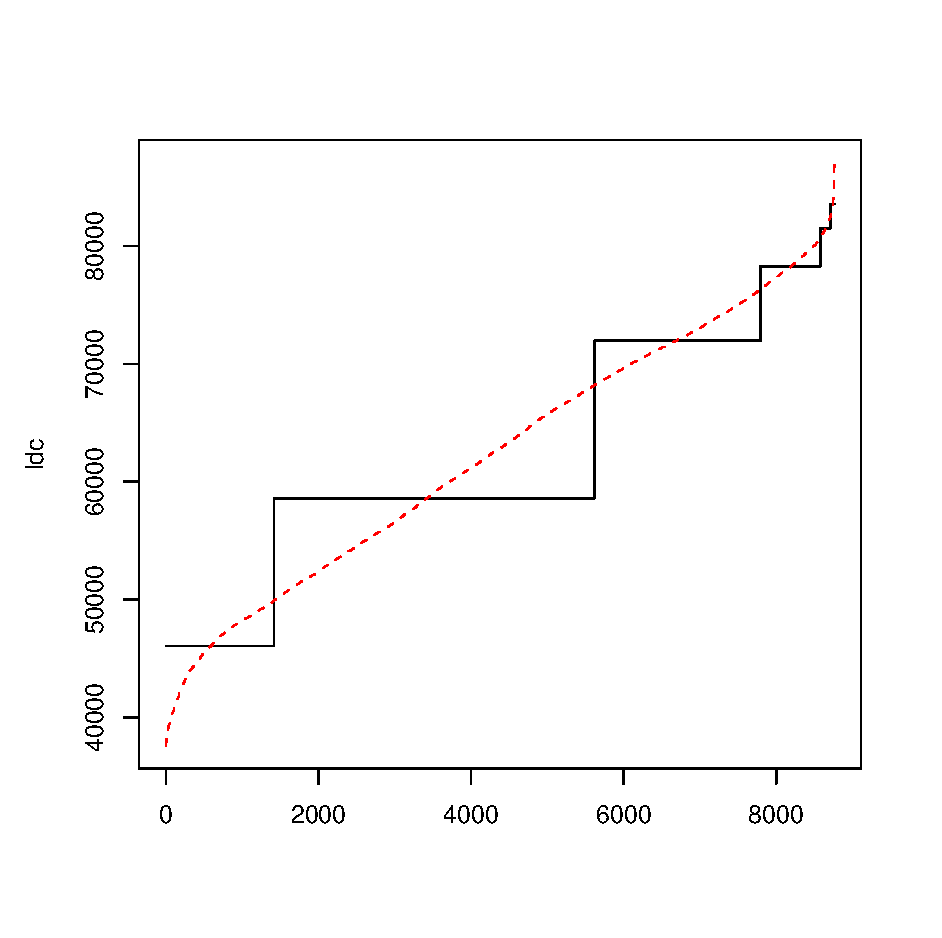
\includegraphics[width=.5\textwidth]{data/ldc}
      \label{fig:ldc}
      \caption{Load Duration Curve in MW for Austria and Germany}
      source: UCTE\footnote{http://www.ucte.org/}
\end{figure}
Figure \ref{fig:ldc} shows the load duration curve for Germany and Austria. It can be seen that there are a few extreme demand spikes and normal values between roughly 80.000 and 40.000 MWh.. To get a better picture of the market, in Figure \ref{fig:korrelation}, hourly Prices from the EEX were plotted against total hourly electricity load in the economy. The correlation is evident. Furthermore, there seems to be an upper bound to capacity which leads prices to explode if that bound is approached. Of course, quantity is not the only factor to explain prices and so there is uncertainty associated with our model. It could well be that demand in the neighboring countries is lower than expected during a high demand period in Germany and so this free capacities dampen the price spike at the EEX. All these uncertain other developments shall be accounted for by our approximated load duration curve which tells us how often the market is in which state during a year. An interesting thing to note is that if we plot prices and quantities at the EEX there seems to be no correlation at all. This is another sign that the exchange just does not cover the whole market and that there is a closely related OTC market which, together with the exchange forms the actual market for electricity.

\begin{figure}[h]
\centering
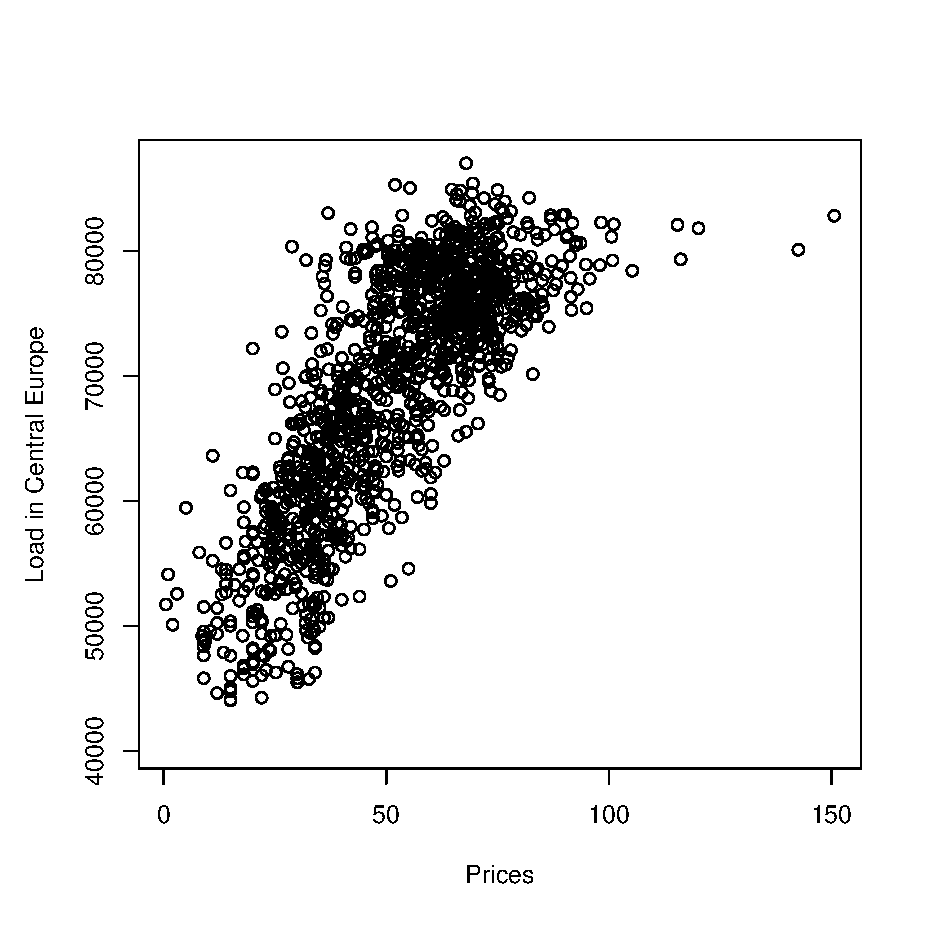
\includegraphics[width=.5\textwidth]{data/korrelation}
      \label{fig:korrelation}
      \caption{Load Duration Curve and our approximation for Austria and Germany}
      source: UCTE and EEX \footnote{http://www.ucte.org/; http://www.eex.com/}
\end{figure}

To account for different states of the market we separated the price-quantity combinaitons which occurred within a year by prices. As can be seen in Table \ref{tab:demand}, markets with extremely high prices occur only seldomly and prices between 20 and 40 are most common. For each of the six states in which the market might be we created linear demand functions based on average prices and quantities in theese states. Average quantities can also be seen in figure \ref{fig:ldc} where the real load duration curve is compared with our approximation. Note that in order to account for price spikes we model the high-price end of the market quite accurately. To construct demand curves, \cite{Neuhoff2005} use a demand elasticity of 0.1, whereby \cite{Genc2007} argue that 0.2 is more commonly used to simulate the electricity market. As we have a more long run focus we decided to use 0.2 as in the long run, elasticity is higher. It might be argued, that in an electricity market, there is no elasticity anyway as maybe only a very few industrial clients reduce their demand as prices rise. Responding to this, \cite{Bushnell2003} notes that imports and exports provide some elasticity.

\begin{table}
\begin{center}
\begin{tabular}{lllll}
\hline
 & \multicolumn{1}{c}{Occurance} & \multicolumn{1}{c}{average price} & \multicolumn{1}{c}{average quantity} &  \\ 
 & \multicolumn{1}{c}{per year} & \multicolumn{1}{c}{(EUR)} & \multicolumn{1}{c}{(MWh)} &  \\ 
 \hline
$>$ 100 & \multicolumn{1}{c}{46} & \multicolumn{1}{c}{128} & \multicolumn{1}{c}{83558} &  \\ 
between 80 and 100 & \multicolumn{1}{c}{134} & \multicolumn{1}{c}{86} & \multicolumn{1}{c}{81493} &  \\ 
between 60 and 80 & \multicolumn{1}{c}{788} & \multicolumn{1}{c}{68} & \multicolumn{1}{c}{78256} &  \\ 
between 40 and 60 & \multicolumn{1}{c}{2174} & \multicolumn{1}{c}{49} & \multicolumn{1}{c}{71956} &  \\ 
between 20 and 40 & \multicolumn{1}{c}{4201} & \multicolumn{1}{c}{30} & \multicolumn{1}{c}{58578} &  \\ 
below 20 & \multicolumn{1}{c}{1417} & \multicolumn{1}{c}{14} & \multicolumn{1}{c}{42627} &  \\
\hline
 & \multicolumn{1}{c}{8760} &  &  &  \\ 
 \hline
\end{tabular}
\end{center}
\label{tab:demand}
\caption{market segments}
\begin{center}
source: UCTE and EEX \footnote{http://www.ucte.org/; http://www.eex.com/}
\end{center}    
\end{table}

\subsection{Supply}

By considering fuel costs and average efficiencies of plants, we calculated variable costs per MWh of the different technologies (see \cite{Leprich2004}). For pump storage plants we used the real option value of peak load electricity which we approximated by the average option price for peak load electricity at the EEX in the year 2006. Fixed costs were obtained from business reports and homepages of the firms hereto. We do not provide fixed costs for the two classes of hydropower as costs there depend heavily on the respective sites. Furthermore, all available sites for significant hydropower plants in central europe seem to be occupied already. The reason why we do not provide prices for oil plants is that this technology is unattractive because of sustained high oil prices. The fixed investment costs we use could also be interpreted as a discounted present value of future yearly costs of capital so our analysis is general concerning this point.

Apart from the dominant players, there is a competitive fringe as well which is a price taker as he cannot influence market prices due to it�s small size. \cite{Neuhoff2005} notes that fringe players could also be modeled to respond to output choices of the strategic players, however we do not account for that.



\begin{table}
\begin{center}
\begin{tabular}{llll}
\hline
 & Variable Costs & Fixed Costs &  \\ 
 
 & \multicolumn{1}{c}{(MWh)} & \multicolumn{1}{c}{(MWh)} &  \\ 
 \hline
Hydro & \multicolumn{1}{c}{0} & \multicolumn{1}{c}{n.a.} &  \\ 
Nuclear & \multicolumn{1}{c}{10.3} & \multicolumn{1}{c}{1760} &  \\ 
Brown Coal & \multicolumn{1}{c}{13.8} & \multicolumn{1}{c}{1196} &  \\ 
Hard Coal & \multicolumn{1}{c}{14.4} & \multicolumn{1}{c}{1050} &  \\ 
CCGT & \multicolumn{1}{c}{19.2} & \multicolumn{1}{c}{550} &  \\ 
Oil & \multicolumn{1}{c}{44} & \multicolumn{1}{c}{n.a.} &  \\ 
Pump Storage & \multicolumn{1}{c}{80} & \multicolumn{1}{c}{n.a.} &  \\ 
\hline
\end{tabular}\end{center}
\label{tab:costs}
\caption{variable and fixed costs}
\begin{center}
source: \cite{Leprich2004} and different Homepages  \footnote{Homepages of RWE, EnBW, EoN and Vattenfall, www.oeko.de and www.izes.de}
\end{center}
\end{table}

Installed Capacities of all dominant players and the competitive fringe are given in table \ref{tab:capacities}. It is striking, that most of the renewable capacities are controlled by fringe players. We constructed a supply curve for the competitive fringe by using the following fourth order polynomial approximation (\ref{eq:19}) of the step wise marginal cost function. The approximation, which weights were obtainded by an OLS Method is illustrated in figure \ref{fig:fringe}.

\begin{equation}
  \label{eq:19}
  C^t_{i} = c_1 + c_2 (\sum_{k=1}^m q^{t,s}_{i,m}) + c_3(\sum_{k=1}^m q^{t,s}_{i,m})^2 + c_4(\sum_{k=1}^m q^{t,s}_{i,m})^3 + (\sum_{k=1}^m q^{t,s}_{i,m})^4
 \end{equation}
 
\begin{figure}[h]
\centering
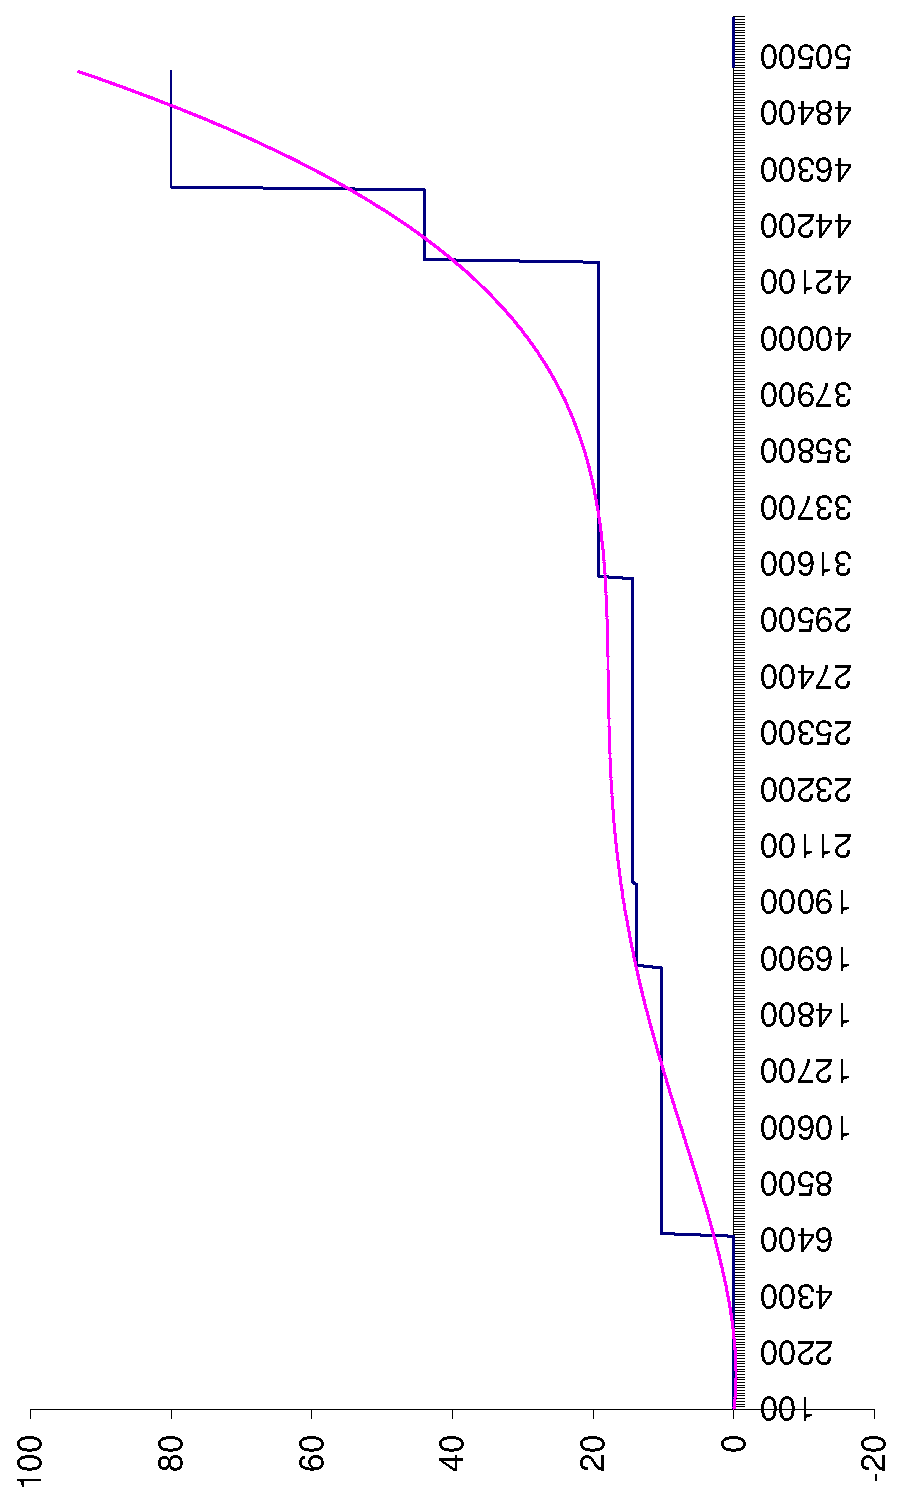
\includegraphics[width=.3\textwidth, angle=-90 ]{data/fringe_costs}
      \label{fig:fringe}
      \caption{polynomial approximation of fringe marginal costs (in EUR and MW)}
      source: own calculations
\end{figure}

For the strategic players however, we cannot use such a simple method because we want to account for the effect of investments in different technologies. The following formulations provide cost functions which are continuous, differentiable and provide a reasonable approximation of step wise cost functions.

\begin{equation}
  \label{eq:20}
		MC^{t}_{i} =  c_m + b \frac{q^{t,s}_{i,m}}{K^{t,s}_{i,m}}^\phi
 \end{equation}

\begin{equation}
  \label{eq:20}
		C^{t}_{i} = \sum_{k=1}^{m} q^{t,s}_{i,m} c_m + \frac{1}{(K^{t,s}_{i,m}-q^{t,s}_{i,m})}
 \end{equation}

With marginal costs

\begin{equation}
  \label{eq:20}
		C^{t}_{i} = \sum_{k=1}^{m} c_m + \frac{1}{(K^{t,s}_{i,m}-q^{t,s}_{i,m})^2}
 \end{equation}





Show that Austrian players are fringe? 

Long term structure of plant parks.

How does the resulting plant park structure look like, if firms actually play two-stage open or closed-looped games and other possible market structures (perfect competition, Betrand). 

How could the current market structures look like one long term step ahead (in ten years from now, one investment cycle).

Welfare implications from different market structures.

Implications of capacity markets.


%\section{Ideas}

\begin{itemize}
	\item \cite{Pineau2003} study how electricity prices, production levels and production capacities unfold in \emph{absence of regulation}. Why test different regulatory measures in this game theoretic setting?
	\item Can transmission pricing and constraints also be ignored in Austria?
	\item Parameters to check in sensitivity analysis: depreciation rate of generating capacity
\end{itemize}



%------------------------------------------------------

\markboth{References}{References} %\frenchspacing
\bibliographystyle{chicago}
%\nocite{*}
\bibliography{microsim}

% \appendix
% \newpage
% \section*{Appendix}
% \input{appendix/notes.tex}
% \input{appendix/units.tex}
% \begin{landscape}

\begin{table}
\scriptsize
\begin{tabular}[h]{ccccc}
\hline
\textbf{Investment problem}\\
\hline
  Authors & Information structure & Solution method & Transmission network & Numerical application \\
\hline
\cite{Genc2007} & $S$-adapted open-loop & MCP & No & electricity market, Ontario, Canada\\
1 & 2 & 3 & 4 & 5 \\
\hline
\textbf{Stochastic oligopoly models}\\
\hline
\cite{Salant1982}\\
\cite{Wolf1997}\\
\cite{Haurie2001}\\
\cite{Haurie2002}\\
\cite{Murto2004}
\end{tabular}
\end{table}
bla ble blu


\textbf{References:} \cite{Salant1982, Wolf1997, Haurie2001, Haurie2002, Pineau2003, Murto2004}\\


The $S$-adapted information structure was introduced by \cite{Haurie1990}.
$S$-adapted structure is similar to the open-loop case, except that the strategies of the players adapt to the sample path of the stochastic variable \citep[see][pg. 128]{Pineau2003}.

\cite{Haurie2002} developed an approximation method with variational inequalities for $S$-adapted oligopoly equilibria. It can be used with any discrete state process that can be represented as an event tree can be used as description of the random disturbances.

\cite{Murto2004} solves the game with feedback information structure.

\cite{Haurie2001}, \cite{Genc2007}

developed an approximation method with variational inequalities for $S$-adapted oligopoly equilibria. It can be used with any discrete state process that can be represented as an event tree can be used as description of the random disturbances.


Market simulation: \cite{Torre2003}, \cite{Valenzuela2007}, \cite{Hobbs2001},\cite{Otero-Novas2000}

General review paper: \cite{Neuhoff2005}, \cite{Ventosa2005}, \cite{Kahn1998}

\end{landscape}



%%% Local Variables: 
%%% mode: latex
%%% TeX-master: "../emarket_simulation"
%%% End: 

% 
\begin{table}[htb]
\centering
\caption{quantities offered and market prices by different firms in different market states}
% Table generated by Excel2LaTeX from sheet 'Tabelle1'
\begin{tabular}{llrrrrrr}
\hline
\hline
           &            & extr. high &    v. high &       high &    interm. &        low &     v. low \\
\hline
       RWE & Hydro Power &        741 &        741 &        741 &        741 &        741 &        741 \\

           &    Nuclear &       5499 &       5499 &       5499 &       5499 &       5499 &       5499 \\

           &    Lignite &      10554 &      10554 &      10554 &      10554 &      10285 &       3684 \\

           &  Hard Coal &       7249 &       7249 &       6675 &       3124 &            &            \\

           &  {\bf Sum} & {\bf 24043} & {\bf 24043} & {\bf 23469} & {\bf 19918} & {\bf 16525} & {\bf 9924} \\
\hline
       EON & Hydro Power &       1320 &       1320 &       1320 &       1320 &       1320 &       1320 \\

           &    Nuclear &       8473 &       8473 &       8473 &       8473 &       8473 &       8473 \\

           &    Lignite &       1425 &       1425 &       1425 &       1425 &       1425 &        131 \\

           &  Hard Coal &       9461 &       9461 &       9461 &       8700 &       3133 &            \\

           &        Gas &       2340 &       1238 &            &            &            &            \\

           &  {\bf Sum} & {\bf 23019} & {\bf 21917} & {\bf 20679} & {\bf 19918} & {\bf 14351} & {\bf 9924} \\
\hline
Vattenfall & Hydro Power &          9 &          9 &          9 &          9 &          9 &          9 \\

           &    Nuclear &       1421 &       1421 &       1421 &       1421 &       1421 &       1421 \\

           &    Lignite &       6932 &       6932 &       6932 &       6932 &       6932 &       6932 \\

           &  Hard Coal &       1729 &       1729 &       1729 &       1729 &       1729 &            \\

           &        Gas &        870 &        870 &        870 &        870 &            &            \\

           &        Oil &       1429 &       1429 &       1429 &        702 &            &            \\

           &   Pump St. &       2883 &        702 &            &            &            &            \\

           &  {\bf Sum} & {\bf 15273} & {\bf 13092} & {\bf 12390} & {\bf 11663} & {\bf 10091} & {\bf 8362} \\
\hline
      EnBW & Hydro Power &        447 &        447 &        447 &        447 &        447 &        447 \\

           &    Nuclear &       4272 &       4272 &       4272 &       4272 &       4272 &       4272 \\

           &    Lignite &        453 &        453 &        453 &        453 &        453 &        453 \\

           &  Hard Coal &       3288 &       3288 &       3288 &       3288 &       3288 &       1465 \\

           &        Gas &       1083 &       1083 &       1083 &       1083 &            &            \\

           &        Oil &        617 &        617 &        617 &        617 &            &            \\

           &   Pump St. &        368 &        368 &            &            &            &            \\

           &  {\bf Sum} & {\bf 10528} & {\bf 10528} & {\bf 10160} & {\bf 10160} & {\bf 8460} & {\bf 6637} \\
\hline
           &    ov. Sum & {\bf 72863} & {\bf 69580} & {\bf 66698} & {\bf 61660} & {\bf 49427} & {\bf 34847} \\
\hline
           &      Price &  {\bf 210} &  {\bf 149} &  {\bf 118} &   {\bf 83} &   {\bf 52} &   {\bf 27} \\
\hline
\hline
\end{tabular}
\label{tab:statquant}
\begin{center}
Source: own calculations
\end{center}
\end{table}

\clearpage
\newpage
%\vspace{3cm}
\begin{table}[htb]
\centering
\caption{shadow prices of capacity, separated by technologies and market states}
% Table generated by Excel2LaTeX from sheet 'Tabelle1'
\begin{tabular}{llrrrrrrr}
\hline
           &            & extr. high &    v. high &       high &    interm. &        low &     v. low &  {\bf Sum} \\
\hline
       RWE & Hydro Power &        831 &       1970 &       6698 &      18479 &      12603 &       4251 & {\bf 44832} \\

           &    Nuclear &        743 &       1715 &       5201 &      14348 &       4621 &       1559 & {\bf 28188} \\

           &    Lignite &        693 &       1568 &       4334 &      11957 &            &            & {\bf 18552} \\

           &  Hard Coal &        440 &        831 &            &            &            &            & {\bf 1271} \\
\hline
       EON & Hydro Power &       1191 &       3471 &      16261 &      18479 &      35709 &       4251 & {\bf 79362} \\

           &    Nuclear &       1104 &       3216 &      14764 &      14348 &      27727 &       1559 & {\bf 62718} \\

           &    Lignite &       1053 &       3069 &      13897 &      11957 &      23106 &            & {\bf 53082} \\

           &  Hard Coal &        800 &       2332 &       9563 &            &            &            & {\bf 12695} \\
\hline
Vattenfall & Hydro Power &       3917 &       9702 &      44668 &      79134 &      81002 &       7954 & {\bf 226377} \\

           &    Nuclear &       3830 &       9447 &      43171 &      75003 &      73020 &       5262 & {\bf 209733} \\

           &    Lignite &       3779 &       9300 &      42304 &      72612 &      68399 &       3703 & {\bf 200097} \\

           &  Hard Coal &       3526 &       8563 &      37970 &      60655 &      45293 &            & {\bf 156007} \\

           &        Gas &       2726 &       6231 &      24259 &      22827 &            &            & {\bf 56043} \\

           &        Oil &       2243 &       4824 &      15985 &            &            &            & {\bf 23052} \\

           &   Pump St. &        587 &            &            &            &            &            &  {\bf 587} \\
\hline
      EnBW & Hydro Power &       5587 &      11512 &      52311 &      90176 &      98341 &      12045 & {\bf 269972} \\

           &    Nuclear &       5500 &      11257 &      50814 &      86045 &      90359 &       9352 & {\bf 253328} \\

           &    Lignite &       5449 &      11110 &      49947 &      83654 &      85738 &       7794 & {\bf 243692} \\

           &  Hard Coal &       5196 &      10373 &      45613 &      71697 &      62633 &            & {\bf 195512} \\

           &        Gas &       4396 &       8041 &      31902 &      33869 &            &            & {\bf 78208} \\

           &        Oil &       3913 &       6634 &      23628 &      11042 &            &            & {\bf 45217} \\

           &   Pump St. &       2257 &       1810 &            &            &            &            & {\bf 4067} \\
\hline
\hline
\end{tabular}  
\label{tab:statlambda}
\begin{center}
Source: own calculations
\end{center}
\end{table}
\end{document}

%%% Local Variables: 
%%% mode: latex
%%% TeX-master: t
%%% End: 
